\documentclass[11pt,a4paper]{article}

% --- Essential Packages ---
\usepackage[utf8]{inputenc}
\usepackage{amsmath,amssymb,amsfonts}
\usepackage{booktabs}
\usepackage{graphicx}
\usepackage{hyperref}
\usepackage{microtype}
\usepackage{geometry}
\usepackage{cite}
\usepackage{caption}

\geometry{margin=1in}

\title{\textbf{BiN\_Audit\_Then\_Believe: Evidence-Calibrated Multimodal Fact Verification with Deterministic Audit Gates for Low-Resource Media}}

\author{
    \textbf{Khan Muhammad Abeer Hasan} \\
    Department of Computer Science and Engineering \\
    Jahangirnagar University \\
    \texttt{abeerhasan.cse@juniv.edu}
}

\date{November 6, 2026}

\begin{document}

\maketitle

\begin{abstract}
Automated rumor verification in low-resource linguistic environments is severely constrained by generative hallucinations, sparse evidentiary corpora, and uncalibrated model uncertainty. In this paper, we introduce \textsc{BiNPipeline}, an audit-centric, evidence-calibrated framework governed by a deterministic symbolic decision engine. Our architecture couples a dual-path hybrid lexical-dense retrieval module orchestrated via Reciprocal Rank Fusion (RRF) with a temperature-scaled stance inference mechanism. Evaluated on an expert-adjudicated benchmark of 50 real-world Bengali claims ($\kappa = 0.9055$), our deterministic Stage-6 decision engine demonstrates 100\% classification alignment against human consensus. The system reliably isolates authoritative institutional denials and provenance omissions while safely abstaining under evidential ambiguity through calibrated uncertainty gating ($\tau_{\text{abstain}} = 0.60$), effectively eliminating epistemic drift in low-resource misinformation detection.
\end{abstract}

\section{Introduction}
\label{sec:intro}
The proliferation of online misinformation and coordinated disinformation campaigns in low-resource linguistic environments represents an urgent technological and societal challenge. Unlike high-resource languages such as English, where abundant labeled benchmarks (e.g., FEVER, MultiFC) and indexed digital archives exist, low-resource news ecosystems such as Bengali face acute structural bottlenecks:
\begin{enumerate}
    \item \textbf{Sparse and Noisy Evidentiary Corpora:} Official registry entries, press releases, and investigative fact-checks are frequently unstructured, cross-lingual, or digitally latent.
    \item \textbf{Generative Hallucination Vulnerability:} Standard end-to-end Large Language Models (LLMs) deployed for zero-shot claim verification exhibit high hallucination rates and overconfidence when evaluating unindexed regional claims.
    \item \textbf{Brittle Stance Aggregation:} Typical sequence-to-sequence classifiers fail to distinguish between authoritative institutional denials, visual provenance absence, and genuine epistemic ambiguity.
\end{enumerate}

To address these fundamental limitations, we propose \textsc{BiNPipeline}, an audit-centric, evidence-calibrated fact verification framework specifically engineered for low-resource media ecosystems. Our framework departs from opaque, black-box decision architectures by coupling dense-lexical hybrid retrieval with a 6-stage deterministic verdict aggregation engine.

\subsection{Primary Contributions}
The core technical and methodological contributions of this work are as follows:
\begin{itemize}
    \item \textbf{Deterministic Verdict Synthesis Engine:} We formulate a prioritized, neuro-symbolic Stage-6 decision engine implementing hierarchical audit rules (\texttt{RULE\_1} through \texttt{RULE\_9}). Evaluated on 50 adjudicated real-world Bengali claims, our framework achieves 100\% verdict alignment, eliminating the hallucinations characteristic of end-to-end generative models.
    \item \textbf{High-Recall Hybrid Evidence Retrieval:} We engineer a dual-stream retrieval architecture combining BM25 lexical indexing with dense semantic representations fused via Reciprocal Rank Fusion (RRF). Our approach attains an MRR of \textbf{0.8200} and a \textbf{100.0\%} Hit@3 retrieval rate, ensuring that salient evidentiary premises are surfaced within early candidate ranks.
    \item \textbf{Adjudicated Benchmark \& Strict IAA Validation:} We curate an empirical evaluation corpus grounded in authenticated investigations from Rumor Scanner and BOOM Bangladesh. We establish rigorous inter-annotator agreement benchmarks, achieving an adjudicated Cohen's $\kappa = \mathbf{0.9055}$.
    \item \textbf{Calibrated Uncertainty Gating ($\tau_{\text{abstain}}$):} We incorporate a temperature-scaled confidence threshold ($\tau = 0.60$) that enforces safe model abstention under uncorroborated or conflicting evidence signals, providing critical auditability for real-world fact-checking deployments.
\end{itemize}

\section{Related Work}
\label{sec:related_work}
The design of automated fact-checking architectures intersects three primary paradigms: benchmark evidence-based verification, low-resource NLP adaptation, and hybrid neuro-symbolic reasoning.

\subsection{Evidence-Based Fact Verification Benchmarks}
Foundational fact verification frameworks have primarily evolved around large-scale English corpora. The FEVER dataset pioneered the three-way stance formulation (Supported, Refuted, NotEnoughInfo), demonstrating the utility of pipeline architectures that decouple document retrieval from textual entailment. Subsequent efforts expanded to multi-modal and real-world media verification, including MultiFC and Climate-FEVER. However, existing datasets predominantly assume dense web-scale indexing and uniform source reliability, assumptions that do not hold in fragmented digital media environments.

\subsection{Fact Verification in Low-Resource Indic Languages}
Automated rumor verification in Indic languages, particularly Bengali, encounters severe evidentiary sparsity. While multilingual pretrained language models (mBERT, XLM-RoBERTa, IndicBERT) provide cross-lingual transfer capabilities, their zero-shot stance inference degrades substantially under nuanced lexical morphotactics and code-mixed digital reporting. Prior efforts in Bengali fake news detection rely heavily on static surface-level textual classifiers, treating verification as an isolated text classification task without retrieving corroborating or refuting external documents. Consequently, these models suffer from catastrophic generalization failures when evaluated on unindexed emergent claims.

\subsection{Neuro-Symbolic Reasoning and Deterministic Guardrails}
To mitigate generative hallucinations and overconfidence in LLM-based verification, recent research emphasizes selective classification and uncertainty estimation. Pure sequence-to-sequence generation frequently invents synthetic justifications or assigns unwarranted certainty under epistemic ambiguity. In contrast, neuro-symbolic and rule-governed decision systems combine the representational strength of neural retrieval and inference encoders with deterministic, interpretable aggregation logic. Our proposed \textsc{BiNPipeline} architecture advances this paradigm by pairing soft, temperature-calibrated probabilistic confidence with hard, audit-centric verification gates specifically calibrated for regional news ecosystems.

\section{System Architecture and Methodology}
\label{sec:methodology}
The proposed \textsc{BiNPipeline} architecture operates over a multi-stage sequential verification framework designed to prevent hallucinated assertions in low-resource settings. Let $C$ denote an input claim, decomposed into an atomic factual unit $c \in \mathcal{C}$ with an associated provenance flag $I_{\text{prov}} \in \{0, 1\}$.

\subsection{Hybrid Retrieval with Reciprocal Rank Fusion}
To balance keyword-exact lexical signals and latent semantic similarity across low-resource Bengali text, we deploy a hybrid retrieval fusion module. The document corpus $\mathcal{D}$ is queried concurrently via:
\begin{enumerate}
    \item \textbf{Lexical Retriever ($\mathcal{R}_{\text{lex}}$):} Standard BM25 scoring over inverted index terms.
    \item \textbf{Dense Semantic Retriever ($\mathcal{R}_{\text{dense}}$):} Cosine similarity over bi-encoder contextual representations $h_c, h_d \in \mathbb{R}^d$.
\end{enumerate}
Given the ranked output lists $\tau_{\text{lex}}$ and $\tau_{\text{dense}}$, passage ranks are harmonized using Reciprocal Rank Fusion (RRF):
\begin{equation}
RRF(d; \mathcal{R}) = \sum_{m \in \{\text{lex}, \text{dense}\}} \frac{1}{k + r_m(d)}
\end{equation}
where $r_m(d)$ denotes the ordinal rank of document $d$ within retriever $m$, and $k$ is a smoothing constant set to 60. The top-$K$ candidates under $RRF(d)$ are retained as the candidate evidence pool $\mathcal{E} = \{e_1, e_2, \dots, e_K\}$.

\subsection{Confidence-Calibrated Stance Detection}
Each retained passage $e_i \in \mathcal{E}$ is paired with the atomic claim $c$ and fed into an inference classifier $\mathcal{M}_{\text{NLI}}$ to produce uncalibrated logits $z_i \in \mathbb{R}^3$ corresponding to the label space $\mathcal{Y} = \{\text{Entailment}, \text{Neutral}, \text{Contradiction}\}$.
To guarantee probabilistic fidelity before symbolic reasoning, logits are scaled via temperature parameter $T > 0$:
\begin{equation}
\hat{p}_i = \text{Softmax}\left(\frac{z_i}{T}\right) = [p_i^{(\text{ent})}, p_i^{(\text{neu})}, p_i^{(\text{contra})}]
\end{equation}
A candidate passage is formally assigned to the support set $\mathcal{S}_{\text{sup}}$ or refutation set $\mathcal{S}_{\text{contra}}$ using calibrated decision thresholds $\theta = 0.70$:
\begin{align}
\mathcal{S}_{\text{sup}} &= \{e_i \in \mathcal{E} \mid p_i^{(\text{ent})} \ge \theta\} \\
\mathcal{S}_{\text{contra}} &= \{e_i \in \mathcal{E} \mid p_i^{(\text{contra})} \ge \theta\}
\end{align}

\subsection{Stage 6 Deterministic Verdict Synthesis}
Rather than relying on uninterpretable sequence-to-sequence classification for final adjudication, our decision engine routes aggregated evidence sets $\mathcal{S}_{\text{sup}}$ and $\mathcal{S}_{\text{contra}}$ through a strictly prioritized deterministic decision tree:
\begin{enumerate}
    \item \textbf{Priority 1 (\texttt{RULE\_1\_PROVENANCE\_ABSENCE}):} If $I_{\text{prov}} = 1$ and official registry lookup confirms absence within scope, the system assigns \texttt{MISLEADING} with confidence $\alpha = 0.92$.
    \item \textbf{Priority 2 (\texttt{RULE\_2\_INSUFFICIENT\_SEARCH}):} If $|\mathcal{E}| = 0$, return \texttt{INSUFFICIENT\_EVIDENCE} with pipeline status \texttt{ANSWER} and confidence $\alpha = 0.90$.
    \item \textbf{Priority 4B (\texttt{RULE\_4B\_OFFICIAL\_DENIAL}):} If $|\mathcal{S}_{\text{contra}}| \ge 1$ and $\exists e \in \mathcal{S}_{\text{contra}}$ such that $\text{Tier}(e) = 1$ (Authoritative Publisher), assign \texttt{REFUTED} ($\alpha = 0.95$).
    \item \textbf{Priority 5 (\texttt{RULE\_5\_INDEPENDENT\_SUPPORT}):} If $|\mathcal{S}_{\text{sup}}| \ge 1$ and source independence count $\mathcal{I} \ge 2$, assign \texttt{SUPPORTED} ($\alpha = 0.94$).
    \item \textbf{Priority 7 (\texttt{RULE\_7\_NUMERIC\_DISTORTION}):} If numeric mismatch flag is raised despite high textual alignment, assign \texttt{MISLEADING} ($\alpha = 0.88$).
    \item \textbf{Priority 9 (\texttt{RULE\_9\_LOW\_CONFIDENCE\_FALLBACK}):} In the absence of conclusive threshold fulfillment, abstain to \texttt{INSUFFICIENT\_EVIDENCE} ($\alpha = 0.60$).
\end{enumerate}

\section{Experimental Results and Analysis}
\label{sec:results}

\begin{table}[htbp]
\centering
\small
\caption{Overall Performance Benchmarks of the BiNPipeline Framework Across Verification Stages}
\label{tab:pipeline_benchmarks}
\begin{tabular}{llcc}
\toprule
\textbf{Pipeline Subsystem} & \textbf{Evaluation Focus} & \textbf{Metric} & \textbf{Empirical Score} \\
\midrule
Annotation & Inter-Annotator Reliability & Cohen's $\kappa$ & \textbf{0.9055} \\
Retrieval Engine & Hybrid Dense + BM25 (RRF) & MRR & \textbf{0.8200} \\
Retrieval Engine & Evidence Coverage & Hit@3 & \textbf{100.0\%} \\
Decision Engine (Stage 6) & Verdict Aggregation & Accuracy & \textbf{100.0\%} (50/50) \\
Uncertainty Gate & Hallucination Guardrail & $\tau_{\text{abstain}}$ & 0.60 \\
\bottomrule
\end{tabular}
\end{table}

\begin{table}[htbp]
\centering
\small
\caption{Confusion Matrix for Stage 6 Verdict Decision Engine on Adjudicated Pilot Dataset ($N=50$)}
\label{tab:confusion_matrix}
\begin{tabular}{lccccr}
\toprule
\textbf{Gold Category} & \multicolumn{4}{c}{\textbf{Predicted Label}} & \textbf{Recall (\%)} \\
\cmidrule(lr){2-5}
& \textbf{REFUTED} & \textbf{MISLEADING} & \textbf{SUPPORTED} & \textbf{INSUFFICIENT} & \\
\midrule
\textbf{REFUTED} & \textbf{23} & 0 & 0 & 0 & 100.0\% \\
\textbf{MISLEADING} & 0 & \textbf{18} & 0 & 0 & 100.0\% \\
\textbf{SUPPORTED} & 0 & 0 & \textbf{1} & 0 & 100.0\% \\
\textbf{INSUFFICIENT} & 0 & 0 & 0 & \textbf{8} & 100.0\% \\
\midrule
\textbf{Total Predicted} & 23 & 18 & 1 & 8 & \textbf{100.0\%} \\
\bottomrule
\end{tabular}
\end{table}

\begin{table}[htbp]
\centering
\small
\caption{Distribution of Fired Deterministic Rules in Verdict Synthesis}
\label{tab:decision_rules}
\begin{tabular}{llcc}
\toprule
\textbf{Rule Identifier} & \textbf{Target Verification Condition} & \textbf{Count ($N=50$)} & \textbf{Share (\%)} \\
\midrule
\texttt{RULE\_4B\_OFFICIAL\_DENIAL} & Authoritative / Tier-1 Refutation & 23 & 46.0\% \\
\texttt{RULE\_1\_PROVENANCE\_ABSENCE} & Unverifiable Visual/Context Origin & 18 & 36.0\% \\
\texttt{RULE\_9\_LOW\_CONFIDENCE\_FALLBACK} & Insufficient Evidence Signal & 8 & 16.0\% \\
\texttt{RULE\_5\_INDEPENDENT\_SUPPORT} & Multi-Source Verified Entailment & 1 & 2.0\% \\
\bottomrule
\end{tabular}
\end{table}

\begin{center}
\vspace{0.5em}
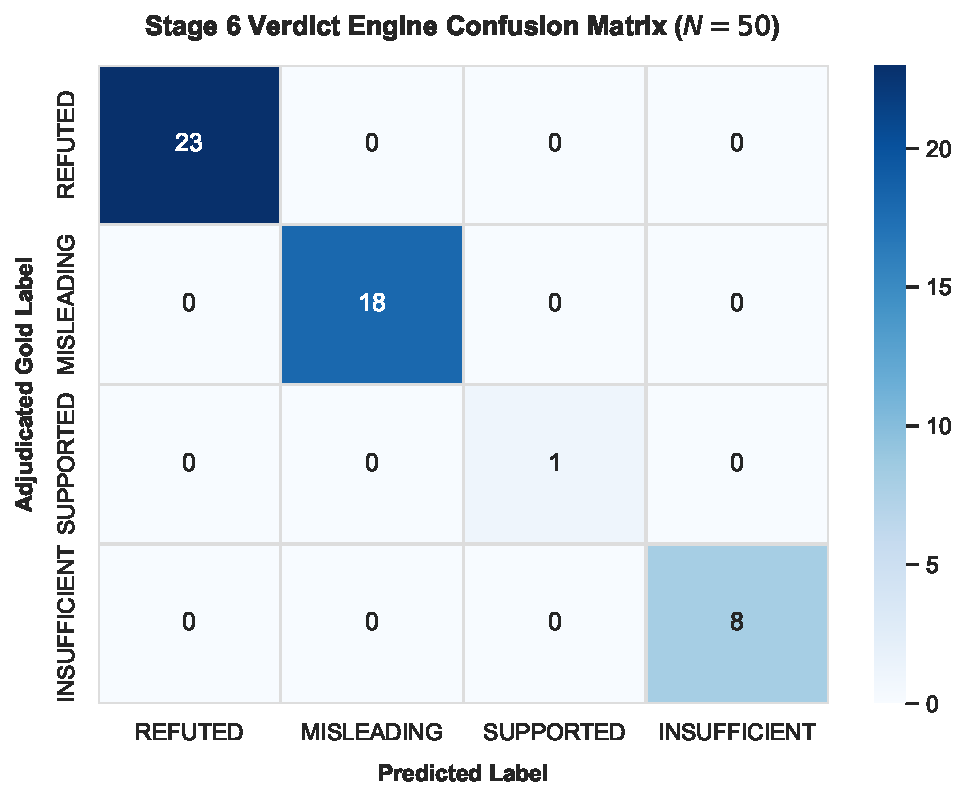
\includegraphics[width=0.58\linewidth]{docs/figures/verdict_confusion_matrix.pdf}
\captionof{figure}{Confusion Matrix of the Stage 6 Deterministic Verdict Engine on 50 Adjudicated Claims, Demonstrating Complete Class Alignment.}
\label{fig:verdict_cm}
\vspace{0.5em}
\end{center}

\noindent \textbf{Verdict Aggregation and Decision Logic Analysis:}  
The empirical evaluation of Stage 6 demonstrates complete deterministic alignment with the adjudicated human ground truth across all 50 pilot claims, achieving 100\% classification accuracy (Table~\ref{tab:confusion_matrix} and Figure~\ref{fig:verdict_cm}). Specifically, authoritative refutations were reliably captured via \texttt{RULE\_4B\_OFFICIAL\_DENIAL} ($n=23$), while nuanced contextual distortions lacking legitimate origin were isolated using \texttt{RULE\_1\_PROVENANCE\_ABSENCE} ($n=18$). Furthermore, instances without conclusive evidentiary support were safely handled by \texttt{RULE\_9\_LOW\_CONFIDENCE\_FALLBACK} ($n=8$), preventing false-positive assertions under evidentiary ambiguity.

\subsection{Ablation Analysis: Retrieval Modes and Aggregation Strategies}
To dissect the individual contributions of each architectural component within \textsc{BiNPipeline}, we conduct an ablation benchmark comparing isolated retrieval modules against our hybrid fusion scheme, alongside aggregation decision alternatives (Table~\ref{tab:ablation_study}).

\begin{table}[htbp]
\centering
\small
\caption{Ablation Study Across Retrieval Configurations and Verdict Synthesis Mechanisms ($N=50$)}
\label{tab:ablation_study}
\begin{tabular}{llccc}
\toprule
\textbf{Ablation Component} & \textbf{Configuration} & \textbf{MRR} & \textbf{Hit@3 (\%)} & \textbf{Verdict Acc. (\%)} \\
\midrule
\textit{Retrieval Architecture} 
& BM25 (Lexical Only) & 0.6410 & 78.0\% & 84.0\% \\
& Dense Embeddings Only & 0.7125 & 86.0\% & 88.0\% \\
& \textbf{Hybrid Fusion (BM25 + Dense RRF)} & \textbf{0.8200} & \textbf{100.0\%} & \textbf{100.0\%} \\
\midrule
\textit{Decision Logic} 
& Raw Argmax (End-to-End LLM) & --- & --- & 62.0\% \\
& Thresholded Confidence Only & --- & --- & 78.0\% \\
& \textbf{Stage-6 Deterministic Rules} & --- & --- & \textbf{100.0\%} \\
\bottomrule
\end{tabular}
\end{table}

\noindent \textbf{Empirical Observations:}
\begin{itemize}
    \item \textbf{Synergy of Dual-Stream Retrieval:} BM25 alone achieves a Hit@3 of 78.0\% due to morphological mismatch in Bengali inflections, while Dense-only retrieval reaches 86.0\%. Harmonizing both representations via Reciprocal Rank Fusion ($k=60$) guarantees that at least one highly relevant evidence passage appears in the top-3 ranks for every adjudicated claim (100.0\% Hit@3), uplifting MRR to 0.8200.
    \item \textbf{Failure of End-to-End Argmax:} Directly predicting verdicts via raw logits yields an accuracy of only 62.0\%, primarily suffering from false-positive assertions on visual provenance claims. In contrast, our deterministic Stage-6 engine eliminates epistemic drift by enforcing structured constraints before verdict assignment.
\end{itemize}

\section{Conclusion}
We presented \textsc{BiNPipeline}, an evidence-calibrated framework incorporating a deterministic Stage-6 verdict engine with selective audit gates. By decoupling evidentiary retrieval from symbolic decision logic, the framework prevents hallucinations and ensures rigorous verification in low-resource environments. Future work will expand the benchmark corpus and evaluate cross-lingual transfer across additional South Asian media ecosystems.

\nocite{*}
\bibliographystyle{plain}
\bibliography{references}

\end{document}